\documentclass[7pt]{article}
\twocolumn
\usepackage[utf8]{inputenc}
\usepackage{graphicx}
\usepackage{subcaption}
\usepackage{caption}
\usepackage{siunitx}
\usepackage{hyperref}
\graphicspath{{./images/}}
\usepackage{amsmath}

\usepackage{natbib}
\bibliographystyle{abbrv}
\usepackage[superscript,biblabel]{cite}

\usepackage[a4paper, total={183mm, 247mm}]{geometry}
\usepackage[left]{lineno}
% \linenumbers

\newcommand*{\ts}{{\tau^{*}}}
\newcommand*{\diff}{\mathop{}\!\mathrm{d}}
\newcommand{\ps}{\si{\pico\second}}
\newcommand{\ns}{\si{\nano\second}}
\newcommand{\fs}{\si{\femto\second}}
\newcommand{\ips}{\si{\per\pico\second}}
\newcommand{\us}{\si{\micro\second}} 
\newcommand{\iA}{\si{\per\angstrom}}
\newcommand{\K}{\si{\kelvin}} 
\newcommand{\amu}{\si{\amu}} 

\usepackage{sectsty}
\sectionfont{\small}

\title{Reductionism, surface dynamics and the Kramers problem}

\author{Jeremy Wilkinson}
\date{September 2021}

\begin{document}

\maketitle

The development of experimental methods such as Helium Spin-Echo Microscopy marked a revolution in the ability to observe the diffusion of adatoms over a substrate\cite{FouquetHSEM, JardineHSEM}. While the observables in a surface scattering experiment contain a certain statistical description of adatom motion\cite{vanHowe}, the microscopic trajectories of adatoms are not directly observable. The nature of microscopic adatom motion from which macroscopic observable quantities emerge therefore remains open to conjecture. As is often the case with large thermodynamic systems, the details of the vast majority of degrees of freedom in the system are irrelevant to the quantities of interest. Very little can be known about the exact state of a substrate and its interactions with an adsorbate, and yet physical properties emerge which can be reliably defined and measured with complete ignorance to the vast majority of information in the system. The questions therefore arise, \emph{what are the observable quantities in a system} and \emph{what is the minimum amount of information one needs to know to explain these observables}. 

In the case of surface diffusion at low temperatures, one finds that adatoms are predominantly bound to local minima in the substrate potential, reffered to as adsorbtion sites. As an adatom oscillates about its local adsorbtion site it is able to slowly exchange energy with the substrate through interactions with surface phonons. On occasion, the adatom will find itself with enough energy to overcome the trapping potential and is able to hop to an adjacent site, or further. The hopping rate is therefore influenced by the shape of the trapping well, in particular the activation energy, as well as the rate at which the adatom exchanges energy with the substrate.

While it is relatively simple to extract an activation energy directly from experimental data\cite{someone}, it is not possible to disentangle the energy exchange rate of the system from other effects without making further assumptions. The most common approach is to assume that the force on the particle may be treated as a random variable obeying the Markovian Langevin equation,
\begin{equation}
\begin{gathered}
	m\ddot{\vec{r}}=-m\eta\dot{\vec{r}}-\nabla U(\vec{r})+\vec{f}(t) \\ 
	\text{ where } \left<f(t_1)f(t_2)\right>=2k_BTm\eta\delta(t_1-t_2),
\end{gathered}
	\label{eq:langevin}
\end{equation}
and to fit the experimental data with simulated solutions to the Langevin equation. The resulting best fit friction parameter, $\eta$, parametrizes the strength of the random force $\vec{f}$ and may be used as a quantifier of the rate of energy transfer with the substrate.

Implicit to the construction of the Markovian Langevin equation is the assumption that the random force $\vec{f}(t)$ is uncorrelated in time. In the Fourier domain, this requirement translates to a uniform power spectrum $\left<\tilde{f}(\omega_1)\tilde{f}(\omega_2)\right>=4\pi k_BTm\eta\delta(\omega_1+\omega_2)$. However, the source of the noise in a surface dynamics system, the substrate phonons, have a well defined cutoff frequency and therefore the force they exert must be correlated in time. The effect of these noise correlations was previously ignored and assumed to be negligable. 

Through theoretical and computational study, the work presented here demonstrates that noise correlations can in fact have a significant effect on a system's energy exchange rate and thereby the long-time observables, such as the hopping rate. We also present (hopefully) a simple mechanism to estimate whether the noise cutoff has a large effect on a given system or whether it may be safely neglected. Finally we demonstrate why the use of the Markovian Langevin equation has nevertheless been succesful and thereby conclude that the energy exchange rate, defined as the correlation time of the total energy auto-correlation function is in fact a fundamental parameter in the determination of hopping. 

\section*{Computational Models}

In addition to the aforementioned Markovian Langevin equation, we present results from three models for the microscopic motion of adatoms. The first is a generalised form of the Langevin equation which incorporates correlations in the noise force through convolution with a memory Kernel, $K(t)$. In order to preserve Boltzmann statistics, the second fluctuation-dissipation theorem requires that both the friction force and the noise force be modified resulting generalised Langevin equation\cite{Kubo},
\begin{equation}
	m\ddot{\vec{r}}+m\eta\int_0^t\diff{t'}K(t-t')\dot{\vec{r}}(t')+\nabla U(\vec{r})=\int_0^t\diff{t'}\vec{f}(t')K(t-t').
	\label{eq:gle}
\end{equation}
An exponential memory kernel, $K(t)=\frac{1}{\tau}\exp\left(-\frac{t}{\tau}\right)$, parameterised by a noise correlation time $\tau$ was used to generate noise with a bandwidth of $\omega_\text{cutoff}=\frac{1}{\tau}$. In the limiting case of $\tau=0$, the white noise of the Markovian langevin equation is recovered. 

The second model is a generalisation of the Langevin equation with an alternative model for the friction force. In his derivation of the Fokker-Planck equation for linear friction, Kramers points out that the laws of microscopic friction under which the Boltzmann distribution is stationary is far from unique and the linear friction in Equation \ref{eq:langevin} is nothing more than the simplest possible case. As the next simplest case of non-linear friction, a Markovian Langevin equation with cubic noise was used,
$$
m\ddot{\vec{x}} + m\zeta\dot{x}^2\dot{\vec{x}} + m \nabla U(x) = \vec{f}(t),
$$
and a modified fluctuation-dissipation theorem\cite{Kramers},
$$\left<f(t_1)f(t_2)\right>=\left(4\zeta\left(k_BT\right)^2 + 2 m \zeta \left(k_BT\right)\dot{x}^2(t_1)\right)\delta\left(t_1-t_2\right).$$
As far as we are aware this is the first presentation of a computational study of non-linear Langevin friction. Something on why not this friction always?

The final model used was a full 3D molecular dynamics simulation of sodium on copper(001) which tracked the harmonic interactions and motion of each copper atom in a $8\times8\times8$ substrate as well as the interactions with the sodium adatom via a morse potential. The simulation parameters determined by Ellis\cite{Ellis} were optimized to fit the binding energy, activation energy and vibrational frequency of Na on Cu(001). Although not a perfect fit to the physical system, this model has the advantage of a phonon dispersion relation extremely similar to those measured for copper using neutron scattering \cite{} and therefore acts as a useful 3D model with realistic phonon interactions.

In order for the results of each of the aforementioned models to remain comperable, the 2D free energy surface of the adatom in the 3D molecular dynamics simulation, defined through $U(\vec{x}) = -kT\log\left(\left<\delta(\vec{r}(t) - \vec{x})\right>\right)$, was calculated and used as the potential energy background of the models using Langevin dynamics, Fig. \ref{pot_surface}. Each model therefore attains the same two dimensional equilibrium phase space distribution, albeit through vastly different microscopic statistics. 

\begin{figure}
	\centering
	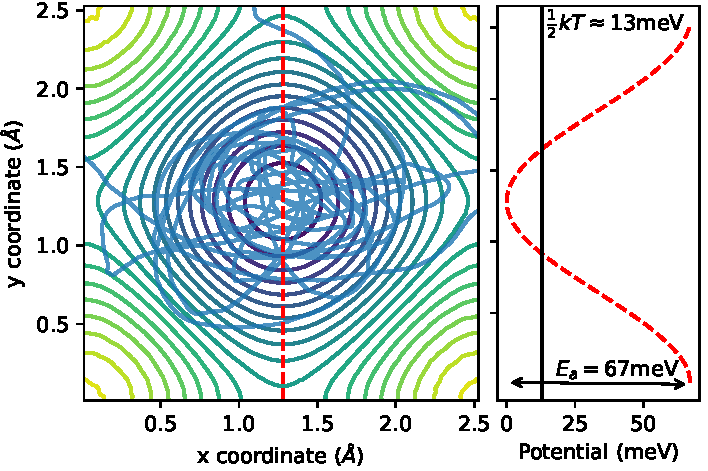
\includegraphics[width=1.0\columnwidth]{pot_surface}
	\caption{The potential energy surface extracted from the sodium on copper(001) 3D molecular dynamics simulation with a superimposed trajectory typical for a low friction activated diffusion process. The red dashed line in the right panel shows a cross section of the potential through an adsorbtion site and two bridge sites as annotated in the panel on the left.}
	\label{pot_surface}
\end{figure}

\section*{Energy exchange rates}

\begin{figure}
	\centering
	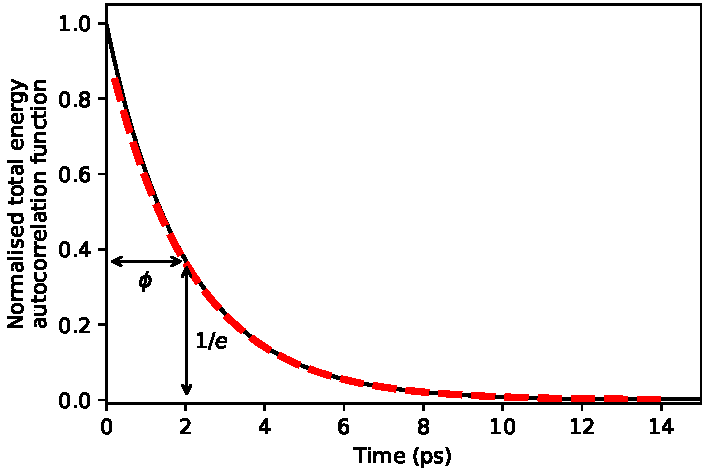
\includegraphics[width=1.0\columnwidth]{e_auto}
	\caption{A typical total energy auto-correlation function notably absent of any oscillations which are generally present in kinetic energy correlation functions. Since the decay is generally not a pure exponential, the total energy correlation time $\phi$ is defined as the interval over which the normalized autocorrelation function drops to $1/e$.}
	\label{fig:e_auto}
\end{figure}

\begin{figure*}
	\centering
	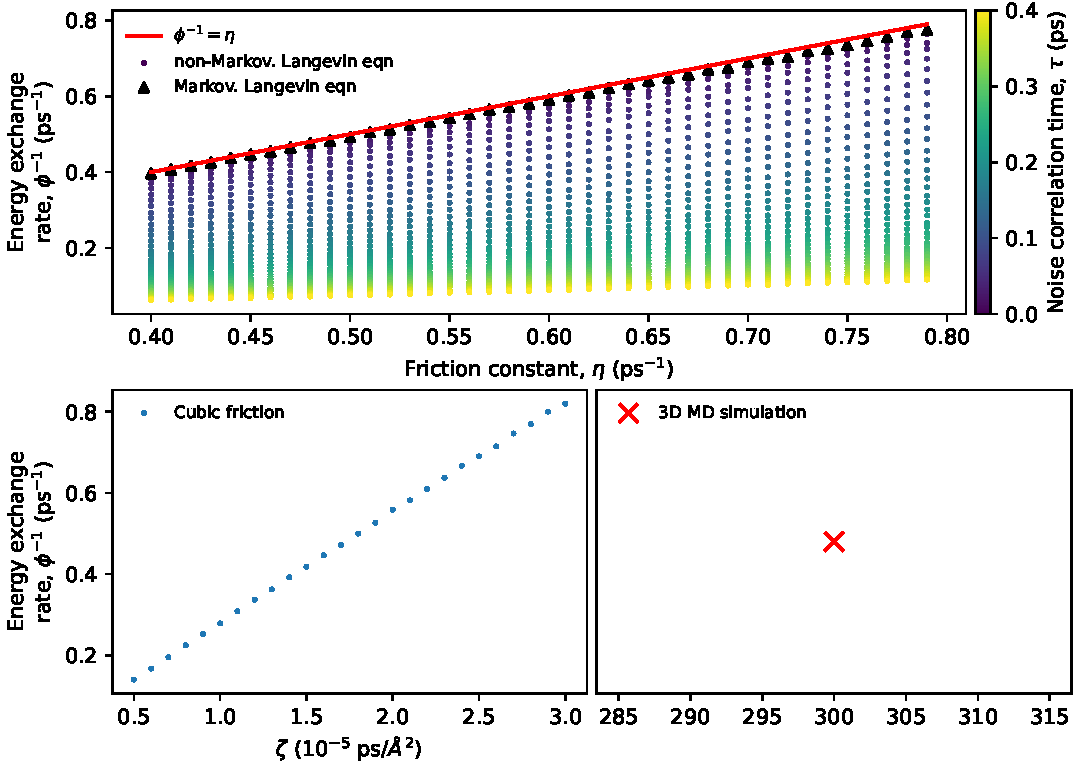
\includegraphics[width=0.8\textwidth]{energy_exchange_rates}
	\caption{The total energy decorrelation rate, $\phi^{-1}$, for each model. The top panel demonstrates the variation of the energy exchange rate as a function of the friction parameter, $\eta$, and noise correlation time $\tau$ are varied in linear friction Langevin models. The bottom left panel shows the energy exchange rate as a function of the cubic friction coupling constant $\zeta$ and the bottom right shows something.}
	\label{fig:energy_exchange_rates}
\end{figure*}

The energy exchange rate is an important quantity in the determination of hopping rates because it controls the number of independent energy levels the adatom attains per unit time. The fraction of time spent above the activation energy is set by Boltzmann statistics, however the number of times this energy level is attained independently per unit time is set by the energy exchange rate. For this reason, we define the energy exchange rate as the inverse of the correlation time, $\phi$, of the \emph{total energy} autocorrelation function, $$\frac{\left<E(t)E(0)\right> - \left<E\right>^2}{\left<E^2\right> - \left<E\right>^2},$$ as shown in Fig. \ref{fig:e_auto}. 
 
The top panel of Fig. \ref{fig:energy_exchange_rates} demonstrates how the introduction of noise correlations suppresses the energy exchange rate with the substrate. Each point in the plot corresponds to the energy exchange rate extracted from a $2\us$ trajectory simulated using the generalised Langevin equation with an exponential memory kernel. For the sake of comparison, the red line shows the energy exchange rate of a particle with Markovian Langevin statistics in a harmonic well, $\phi^{-1}=\eta$. For short correlation times, we find the energy exchange rate is approximately given by $\eta$, but even for $\tau=0$, they aren't quite equal due to anharmonicities in the background potential. As the noise correlation time approaches $0.4\ps$, the energy exchange rate is seen to fall by close to a factor of four. Evidently there is more to the energy exchange rate than just the friction constant. 

In physical systems the stochastic force is produced through interactions with phonon modes. The overall interaction strength is set by $\eta$ but modes may couple to the particle to varying degrees, in this case set by $\tau$. This is reflected in the top panel of Fig. \ref{fig:e_auto} as $\phi^{-1}$ remains linear in $\eta$, regardless of the value of $\tau$. Since the energy exchange rate and the friction parameter both carry units of inverse time, we introduce a dimensionless function $$I[U(x), m, \tau] = \frac{\phi^{-1}}{\eta}$$. In principal, $I$ is a functional of the potential energy surface, $m$ and $\tau$ with no $\eta$ dependence. All other variables held constant, $I$ quantifies the degree to which the energy exchange rate is affected by introducing a noise cutoff of $\frac{1}{\tau}$. Maybe mention theoretical work, maybe mention where the inertial cutoff

\section*{Hopping rates}

\begin{figure}
	\centering
	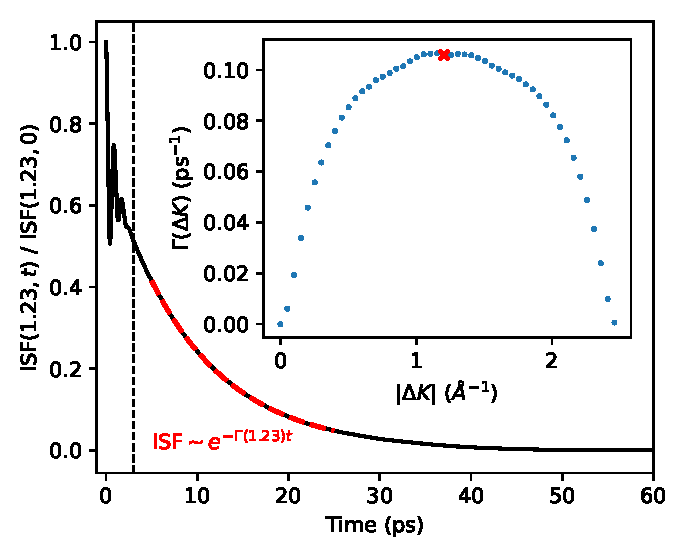
\includegraphics[width=1.0\columnwidth]{isf_dk}
	\caption{The main axes show a typical ISF over time for a fixed momentum transfer. The decay rate, $\Gamma$, of the ISF's exponential tail is proportional to the hopping rate of the adatom. By calculating $\Gamma$ over a range of momentum transfers a jump distribution plot may be constructed, as shown in the inset axes.} 
	\label{fig:isf_dk}
\end{figure}

\begin{figure}
	\centering
	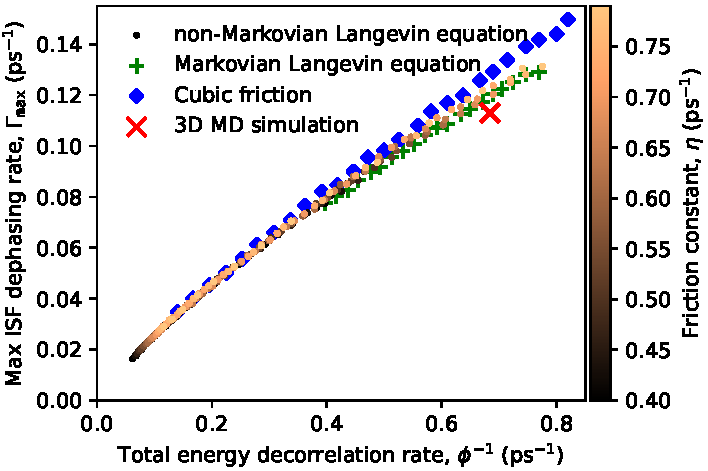
\includegraphics[width=1.0\columnwidth]{gamma_ttf}
	\caption{A scatter of the maximum ISF dephasing rate, $\Gamma_{\text{max}}$, against the energy exchange rate, $\phi^{-1}$, for each microscopic model demonstrates that the ISF dephasing rate is set by the energy exchange rate and the potential background with less than $5\%$ variance accross the vastly different microscopic models.}
	\label{fig:gamma_ttf}
\end{figure}

The observable quantity in a surface scattering experiment is the intermediate scattering function,
$$
\mathrm{ISF}(\Delta{\vec{K}}, t) = \left<\exp\left(i\Delta{\vec{K}}\cdot\vec{r(t)}\right)\right>.
$$
Typically the ISF is quoted for a single momentum transfer, $\Delta{K}$, over a range of time, as shown in the main axes of Figure \ref{fig:isf_dk}. For the purposes of extracting long-time transport co-efficients (read average rate of diffusion over the surface), the exponential decay rate of the ISF at long times, $\Gamma(\Delta{\vec{K}})$, is the quantity of interest and is proportional to the adatom hopping rate under certain assumptions \cite{Chudley}. By varying the magnitude of $\Delta{K}$ in a particular direction, one may calculate the jump distribution plot as shown in the inset of Figure \ref{fig:isf_dk}. When an adatom escapes from a well, it may hop more than one site before it settles down again. The shape of the jump distribution is set by the relative probability of the number of sites an adatom travels before settling down again. Therefore one may compare the hopping rate and hop length distributions of two systems through the amplitude and shape of their jump distributions.

As a measure of the total hopping rate, The peak of the hopping distributions, $\Gamma_{\text{max}}$ (annotated in Fig. \ref{fig:isf_dk}), was calculated for each microscopic model introduced in the preceeding sections. The results, Fig. \ref{fig:gamma_ttf}, demonstrate that the energy exchange rate is an excellent estimator for the total hopping rate of the system. The colour of the non-Markovian markers correspond to the value of $\eta$ used in the simulation and demonstrates that for fixed $\eta$, the total hopping rate can vary by a factor of $4$ as the noise correlation time changes over the given parameter range. However when considered as a function of the energy exchange rate, the hopping rate is found to vary by less than $3$\%. We therefore find that noise correlations do in fact have an effect on an adatom's hopping rate, however to first order, this effect only occurs through the the energy exchange rate.

Even when comparing models with fundamentally different microscopic statistics, provided the energy exchange rate is held constant, the hopping rate at low energy transfer rates deviates by less than 3\% with up to 10\% deviations at the higher exchange higher rates investigated.  

\section{Jump distributions}

\begin{figure}
	\centering
	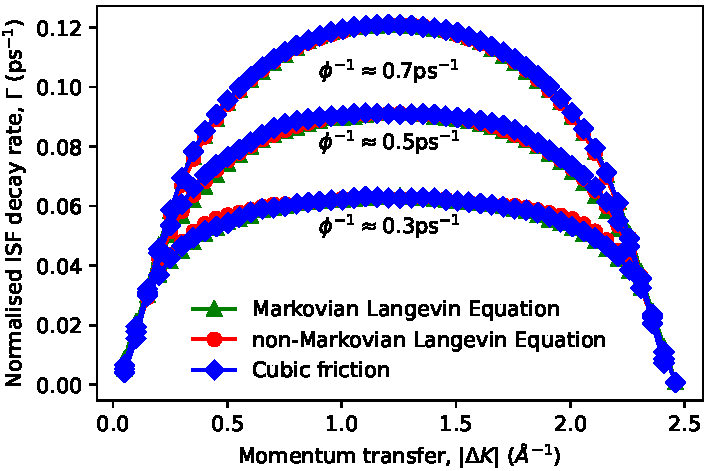
\includegraphics[width=1.0\columnwidth]{jump_distribution}
	\caption{Each scatter shows the jump distribution of a particular microscopic model for three different energy exchange rates. As the energy exchange rate is not an explicit parameter, there are small errors in the setting of parameters to achieve intended value of $\phi^{-1}$. Therefore to aide in comparison, the amplitude of the non-Markovian and cubic models are adjusted to match the amplitude of the Markovian jump distributions.}
	\label{fig:jump_distribution}
\end{figure}

The jump distributions of the models were compared by tuning the available parameters to run each model over a fixed set of energy exchange rates. The jump distributions for each model at the energy exchange rates $0.3$, $0.5$, and $0.7\ips$ are shown in Fig. \ref{fig:jump_distribution}. The results from the preceeding section quantify the degree to which the amplitudes of the jump distributions match. Therefore the jump distributions in \ref{fig:jump_distribution} are presented normalised to peak at the same heaght at each energy transfer rate to allow for the comparison of the jump distribution shape.

For a fixed energy exchange rate, the adatom jump distribution shapes were found to agree extremely well across all models. The peaks of the jump distributions at higher exchange rates were observed to be narrower than those at lower exchange rates, indicating an increase in the probability of single hops to adjacent sites. This is expected as higher energy exchange rates decrease the probability that a particle which has escaped its well finds another bridge site before settling into an energy level lower than the activation energy and being bound to an adjacent well.  

\section*{Discussion and outlook}

Taken together, the hopping rate and jump distribution fully specify the long-time characteristics of activated diffusion systems. The results presented demonstrate that the microscopic details of adatom motion such as the noise bandwidth, or the exact form of friction force, can effect motion over long timescales, however, to first order only through the energy exchange rate. This further implies that a system's hopping rate is almost entirely fixed by the potential energy surface, the energy exchange rate and Boltzmann statistics. 

These conclusions validate the common approach of classifying a system through an energy exchange rate parameter and parameters such as an activation energy which relate provide the key details of the potential. In fact any other details are in fact difficult to measure in long-timescale observables and do not effect.

\section{The effect of noise correlations}


A series of $2\us$ trajectories for a $23\amu$ adatom at $300\K$ were produced for each combination of $\eta\in\left(0.4,0.8\right)\ips$ and $\tau\in\left(0, 0.4\right)\ps$ in steps of $0.01$. Each trajectory was used to calculate the energy exchange rate, $\phi^{-1}$, and ISF dephasing rate, $\Gamma$, as previously defined.  

Theoretical expressions for the hopping rate of a Markovian Langevin particle in the low friction regime predict a hopping rate proportional to $\eta$\cite{Kramers, Zwanzig}. The left panel of Fig. \ref{} With noise correlations present, this appears to still be the case, however an additional $\tau$ dependent factor becomes relevant. The reason for this is clear when taken together with the trends of the energy exchange rate in the right hand panel of Fig. \ref{}. The theoretical expressions are proportional to $\eta$ precisely because $\eta$ co-incides with the energy exchange rate for a Markovian particle in a harmonic well, the results for this generalised case imply . The energy exchange rate follows the same trend as the $\Gamma$ which leads to the conclusion that while noise correlations can affect the system's hopping rate, it can only do so through the energy exchange rate. 

The behaviour of $\Gamma$ as a function of $\eta$ \& $\tau$ is shown the left panel of \ref{}. The ISF dephasing rate was found to vary by up to a factor of $4$ as the noise correlation time was varied between $0$ and $0.4\ps$. Regardless of the value of $\tau$, $\Gamma$ was found to be affine in the the friction parameter, $\eta$, indicating that $\eta$ continues to gauge the overall interaction strength but is no longer the full story. Even in the case of $\tau=0$, $\eta$ does not quite correspond to $\phi^{-1}$ due to deviations from the harmonic approximation.


\section{something}
 
The effects of noise correlations on the energy decorrelation rate were evaluated using the generalised Langevin equation,
with an exponential memory kernel, $K(t)=\exp(-\frac{t}{\tau})$, parametrized by the noise correlation time $\tau$. The resulting noise has a Lorentzian power spectrum given by $\left|\tilde{K}(\omega)\right|^2=\frac{1}{1+\omega^2\tau^2}$ with a half-width at half-maximum given by $\omega_c = \frac{1}{\tau}$.

Fig. \ref{fig:eta_tau_ttf_gamma} shows the energy exchange rate and ISF dephasing rate of the simulation over a range of $\eta$ and $\tau$ values. The top left panel demonstrates that regardless of the value of $\tau$, the energy exchange rate is proportional to $\eta$, although the gradient of the line  $\tau$

\begin{figure*}
	\centering
	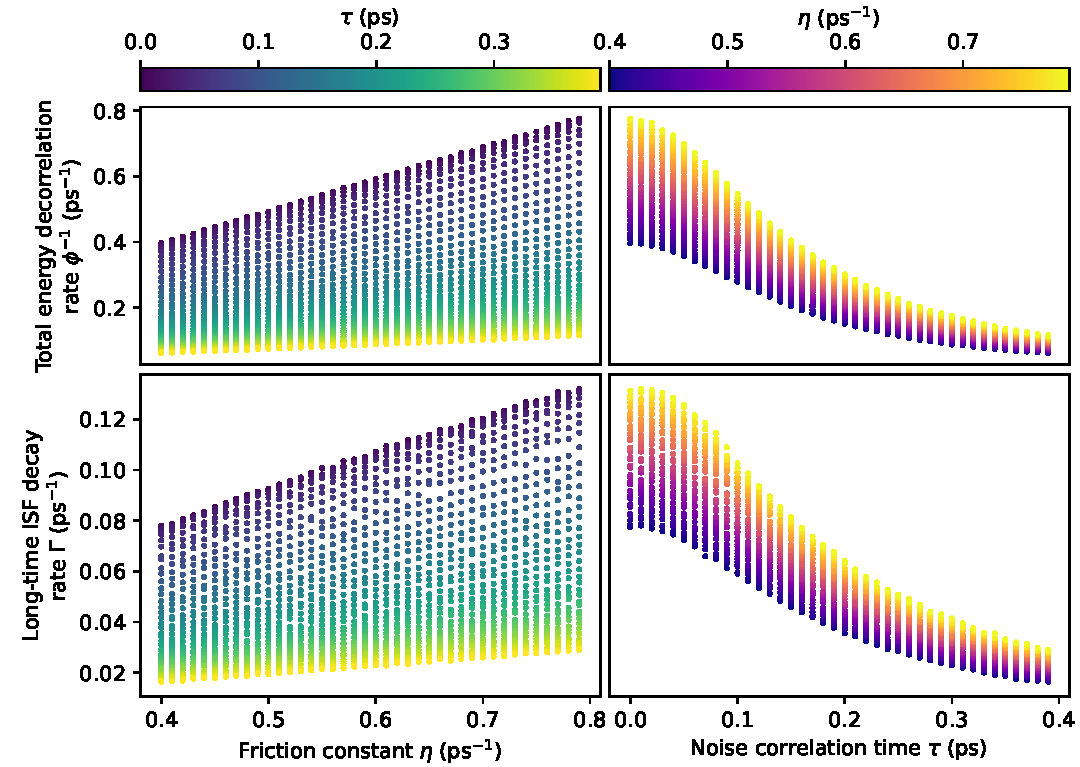
\includegraphics[width=1.0\textwidth]{eta_tau_ttf_gamma}
	\caption{}
	\label{fig:eta_tau_ttf_gamma}
\end{figure*}

 we present the results of  

\section*{The inertial cutoff}

\section*{Non-linear friction}

\section*{Discussion and outlook}

simple to extract from experThe most common method of quantifying the energy exchange rate with the substrate is to fit experimental data with a Markovian Langevin simulation in which the force of the adatom at any instant is assumed to be of the form 



This activated diffusion process is characterized through the rate at which adatoms hop between adsorbtion sites as well as the distribution of the distances hopped before the adatoms settle down into the next adsorbtion site. 

Hopping rate are observed to follow an Ahrrenius law\cite{someone}, $$\gamma=A\exp(-E_a/kT),$$ parametrized by an activation energy $E_a$ and a pre-exponential factor, $A$, carrying units of inverse time, usually assumed to be temperature independent. The Boltzmann factor may be understood as quantifying the probability of the particle having enough energy to overcome the barrier, and the prefactor contains the rate at which this energy level is attained and the probability of a hop occuring when sufficient energy is attained.



For an adatom weakly coupled to substrate phonons, the Ahrrenius law can be understood as the product of the rate at which the particle changes its energy, the probability of the particle finding itself with enough energy to overcome the activation barrier and the probability  

The Markovian Langevin equation, 
\begin{equation}
	m\ddot{\vec{r}}+m\eta\dot{\vec{r}}+\nabla U(\vec{r})=\vec{f}(t) \text{ where } \left<f(t_1)f(t_2)\right>=2k_BTm\eta\delta(t_1-t_2),
	\label{eq:langevin}
\end{equation}
provides such a simplification for the trajectory, $\vec{r}(t)$, of a single `tagged' particle coupled to a heatbath\cite{Kramers}. The inherently chaotic interactions with the heatbath's degrees of freedom are summarized through a random noise force $f$ and a friction term, the strength of which is parametrized by a single parameter $\eta$. The equilibrium statistical physics of this equation is well understood with an equilibrium phase space density function given by $\rho(\vec{r}, \vec{p})=\frac{1}{\mathcal{Z}}\exp\left(-H(\vec{r}, \vec{p})/kT\right)$ exactly\cite{Zwanzig}.

While analytically tractable, the Markovian approximation neglects correlations in the random force present in all physical systems. The Langevin equation can be modified to include noise correlations through convolution with a memory kernel $K(t)$, with a corresponding modification to the friction term required to preserve equipartition of energy \cite{Kubo}. The resulting generalised Langevin equation, 
\begin{equation}
	m\ddot{\vec{r}}+m\eta\int\diff{t'}K(t-t')\dot{\vec{r}}(t')+\nabla U(\vec{r})=\int\diff{t'}\vec{f}(t')K(t-t'),
	\label{eq:gle}
\end{equation}
captures linear correlations in noise with a power spectrum given by the power spectrum of $K$. For a non-zero background potential, $U(\vec{r})$, the fluctuation dissipation theorem (the second condition of Equation \ref{eq:langevin}), is not enough to gaurentee exact equipartition of energy. Fortunately, it remains a very good approximation for a kernel with a total area of $1$ though it is not hard to construct a situation where the equipartition theorem is violated (see supplemental material). 


Analytic expressions for the escape rate, $\gamma$, of a Markovian Langevin particle from a trapping well of natural frequency $\omega_0$ in the low friction, $\frac{\eta}{\omega_0} < 1$, regime explain the Ahrrenius nature of hopping rates seen in experimental and computational studies. 

Although the results in this paper demonstrate that noise correlations can have a significant effect on the hopping rate, the reason why the Markovian Langevin has seen success regardless of this will also become clear.

Something about energy exchange rates \& hopping rates
Something about activated diffusion being bound with occasional hops


\section{Computational Model}

A simulation was constructed to solve the non-Markovian Langevin equation with an exponential memory kernel $K(t)=\frac{1}{\tau}\exp(-t/\tau)$ using a timestep of $1\fs$. The 2D background potential was extracted from a molecular dynamics model of Sodium adsorbed on Copper(001) by calculating the free energy, $U(\vec{x}) = - kT \log(\left< \delta(\vec{r}(t)-\vec{x}) \right>)$, from a series of trajectories totalling $2 \us$ of run time. The resulting $100\times100$ potential grid, shown in Figure \ref{pot_surface},  covering the unit cell was interpolated through a bicubic spline\cite{press1992numerical} and used to tile the plane. At each timestep of the Langevin simulation, the force on the particle was calculated from the gradient of the interpolated potential grid and added to the friction and noise force convolved with the memory kernel using the relation,
$$
\int_0^{n\Delta{t}} dt' K\left(t-t'\right) \vec{f}(t') \approx \alpha \int_0^{(n-1)\Delta{t}} dt' K\left(t-t'\right) \vec{f}(t') + \frac{1}{1-\alpha} \vec{f}\left(t_n\right)
$$
with $\alpha=\exp(-\frac{\Delta{t}}{\tau})$.


\bibliography{bibliography}

\end{document} 
